\documentclass[12pt]{report}
\usepackage{polyglossia} % enable TeX to generate text in target language. Also add support to languages (correct quoting style, etc.)
\setmainlanguage{french}
\usepackage{csquotes} % required to use polyglossia apparently, also handle quotes
\usepackage{fancyvrb} % insert content without interpreting as LaTeX
\usepackage[backend=biber]{biblatex} % bibliography management
\addbibresource{references.bib}
\usepackage[pdfborder={0 0 0.6}]{hyperref} % add hypertext reference support to navigate from and within the document
\usepackage{float} % to correctly position images or any figure environment
\usepackage{graphicx} % manage images
\graphicspath{ {./images/} } % set default path to images
\usepackage{wrapfig}
\restylefloat{figure} % again, to correctly position images or any figure environment
\usepackage{hyperref} % manage URL
\usepackage{appendix} % manage annexe numbering
\usepackage{pdfpages} % to insert pdf

% custom handling of footnotes so I don't have to put them inline or manager counting myself
\newcounter{footnoteMarkCount}
\newcounter{footnoteTextCount}
\newcommand{\fnmark}{\stepcounter{footnoteMarkCount}\setcounter{footnote}{\value{footnoteMarkCount}}\addtocounter{footnote}{-1}\footnotemark}
\newcommand{\fntext}[1]{\stepcounter{footnoteTextCount}\setcounter{footnote}{\value{footnoteTextCount}}\footnotetext{#1}}

\begin{document}
    %%%%%%%%%%%%%%%%%%%%%%%%%%%%%%%%%%%%%%%%%
% University Assignment Title Page
% LaTeX Template
% Version 1.0 (27/12/12)
%
% This template has been downloaded from:
% http://www.LaTeXTemplates.com
%
% Original author:
% WikiBooks (http://en.wikibooks.org/wiki/LaTeX/Title_Creation)
%
% License:
% CC BY-NC-SA 3.0 (http://creativecommons.org/licenses/by-nc-sa/3.0/)
%
% Instructions for using this template:
% This title page is capable of being compiled as is. This is not useful for
% including it in another document. To do this, you have two options:
%
% 1) Copy/paste everything between \begin{document} and \end{document}
% starting at \begin{titlepage} and paste this into another LaTeX file where you
% want your title page.
% OR
% 2) Remove everything outside the \begin{titlepage} and \end{titlepage} and
% move this file to the same directory as the LaTeX file you wish to add it to.
% Then add \input{./title_page_1.tex} to your LaTeX file where you want your
% title page.
%
%%%%%%%%%%%%%%%%%%%%%%%%%%%%%%%%%%%%%%%%%
\begin{titlepage}

    \pagenumbering{gobble} % titlepage is not numbered

    \newcommand{\HRule}{\rule{\linewidth}{0.5mm}} % commmand to make horizontal lines

    \center

    %----------------------------------------------------------------------------------------
    %	HEADING SECTIONS
    %----------------------------------------------------------------------------------------

    \textsc{\LARGE IFOSUP}\\[0.5cm]
    \textsc{\large Institut de Formation Supérieure de la Ville de Wavre}\\[1.5cm]
    \textsc{\Large Bachelier en informatique de gestion}\\[0.5cm]
    \textsc{\large Épreuve intégrée}\\[0.5cm]

    %----------------------------------------------------------------------------------------
    %	TITLE SECTION
    %----------------------------------------------------------------------------------------

    \HRule \\[0.4cm]
    { \huge \bfseries Click and Run}\\[0.4cm]
    \textsc{\large Une application web modulaire pour automatiser les tâches récurrentes}\\[0.5cm]
    \HRule \\[1.5cm]

    %----------------------------------------------------------------------------------------
    %	AUTHOR SECTION
    %----------------------------------------------------------------------------------------

    \begin{minipage}{0.4\textwidth}
        \begin{flushleft} \large
        \emph{Auteur:}\\
        Adrien \textsc{Horgnies}
        \end{flushleft}
    \end{minipage}
    ~
    \begin{minipage}{0.4\textwidth}
        \begin{flushright} \large
        \emph{Directeur de projet:} \\
        Grégory \textsc{Schiano}
        \end{flushright}
    \end{minipage}\\[2cm]

    %----------------------------------------------------------------------------------------
    %	DATE SECTION
    %----------------------------------------------------------------------------------------

    {\large 2018~-~2019}\\[2cm]

    %----------------------------------------------------------------------------------------

    \vfill

\end{titlepage}
 % title page occupies first page
    \clearpage
\newpage
\pagenumbering{gobble}
\null
\clearpage
 % title page must be followed by an ampty page
    %%%%%%%%%%%%%%%%%%%%%%%%%%%%%%%%%%%%%%%%%
% University Assignment Title Page
% LaTeX Template
% Version 1.0 (27/12/12)
%
% This template has been downloaded from:
% http://www.LaTeXTemplates.com
%
% Original author:
% WikiBooks (http://en.wikibooks.org/wiki/LaTeX/Title_Creation)
%
% License:
% CC BY-NC-SA 3.0 (http://creativecommons.org/licenses/by-nc-sa/3.0/)
%
% Instructions for using this template:
% This title page is capable of being compiled as is. This is not useful for
% including it in another document. To do this, you have two options:
%
% 1) Copy/paste everything between \begin{document} and \end{document}
% starting at \begin{titlepage} and paste this into another LaTeX file where you
% want your title page.
% OR
% 2) Remove everything outside the \begin{titlepage} and \end{titlepage} and
% move this file to the same directory as the LaTeX file you wish to add it to.
% Then add \input{./title_page_1.tex} to your LaTeX file where you want your
% title page.
%
%%%%%%%%%%%%%%%%%%%%%%%%%%%%%%%%%%%%%%%%%
\begin{titlepage}

    \pagenumbering{gobble} % titlepage is not numbered

    \newcommand{\HRule}{\rule{\linewidth}{0.5mm}} % commmand to make horizontal lines

    \center

    %----------------------------------------------------------------------------------------
    %	HEADING SECTIONS
    %----------------------------------------------------------------------------------------

    \textsc{\LARGE IFOSUP}\\[0.5cm]
    \textsc{\large Institut de Formation Supérieure de la Ville de Wavre}\\[1.5cm]
    \textsc{\Large Bachelier en informatique de gestion}\\[0.5cm]
    \textsc{\large Épreuve intégrée}\\[0.5cm]

    %----------------------------------------------------------------------------------------
    %	TITLE SECTION
    %----------------------------------------------------------------------------------------

    \HRule \\[0.4cm]
    { \huge \bfseries Click and Run}\\[0.4cm]
    \textsc{\large Une application web modulaire pour automatiser les tâches récurrentes}\\[0.5cm]
    \HRule \\[1.5cm]

    %----------------------------------------------------------------------------------------
    %	AUTHOR SECTION
    %----------------------------------------------------------------------------------------

    \begin{minipage}{0.4\textwidth}
        \begin{flushleft} \large
        \emph{Auteur:}\\
        Adrien \textsc{Horgnies}
        \end{flushleft}
    \end{minipage}
    ~
    \begin{minipage}{0.4\textwidth}
        \begin{flushright} \large
        \emph{Directeur de projet:} \\
        Grégory \textsc{Schiano}
        \end{flushright}
    \end{minipage}\\[2cm]

    %----------------------------------------------------------------------------------------
    %	DATE SECTION
    %----------------------------------------------------------------------------------------

    {\large 2018~-~2019}\\[2cm]

    %----------------------------------------------------------------------------------------

    \vfill

\end{titlepage}
 % and then a copy of itself (weird, I know)

	% set my own counter so that I can style it however I want
	\setcounter{page}{1}

	\chapter*{Licence}
	\VerbatimInput{LICENSE.txt}
	\clearpage

	% style page number with roman numbers
	\renewcommand{\thepage}{\roman{page}}

	\tableofcontents
	\clearpage

	% style page number with arabic numbers
	\renewcommand{\thepage}{\arabic{page}}

	Au long de ces quatres dernières années, j'ai suivi les études pour acquérir le bachelier en informatique de gestion.
Le développement informatique me donne l'impression que tout peut être automatiser.
Ce présent travail est un argument en faveur de cette assertion.

Je travaille à Altissia depuis deux ans.
Je développe des nouvelles fonctionalités, corrige des bogues et réalise différentes tâches de maintenance.
Cette dernière catégorie m'a toujours intriguée.
Pour la plupart, ce sont des tâches récurrentes et courtes, réalisables en deux jours ou moins.
Mais si on additionne le nombre de fois qu'il faut les effectuer et la perte de temps occasionnée par la latence entre le
besoin et l'accomplissement d'une tâche, elles sont finalement chronophages.

Je pense qu'automatiser ces tâches serait un gain de temps considérable et éviterait les erreurs humaines.


	\chapter{Contexte}
	\label{ch:context}

	    \paragraph{}
Altissia développe des sites web pour apprendre les langues en ligne.
Ces sites web utilisent de très nombreuses sortes de données:
\begin{enumerate}
    \item Questions de test de niveau
    \item Leçons
    \item Activités
    \item Vidéos
    \item Images
    \item Sons
    \item Articles de presses
    \item Quiz
    \item Dictées
    \item etc.
\end{enumerate}
Ces données sont loin d'être figées, elles évoluent pour s'adapter aux intérêts des apprenants, aux évolutions des langues, pour apporter des corrections ou plus généralement pour améliorer l'expérience de l'utilisateur.

Dans un monde idéal, toutes ces données seraient manipulées par des outils dédiés qui modifieraient directement les données sur les sites cibles. Toutefois, afin de satisfaire les exigences et desiderata de nos clients dans les temps impartis, le développement du contenu supplante le développement de son outil d'édition.

\paragraph{}
Toutes ces données prennent presque toujours un format différent entre le moment où elles sont travaillées et le moment où elles sont disponibles sur une plate-forme.
Par exemple, une question d'un test de niveau est représentée par une ligne d'un fichier Excel pour les linguistes qui les éditent mais correspond à plusieurs entrées dans une base de données Elasticsearch pour l'application.

\paragraph{}
Il est donc impératif d'effectuer la conversion entre ces différents formats afin de nourrir les applications.


\section{Le client}
\label{sec:customer}

    \begin{wrapfigure}{L}{0.35\textwidth}
    \centering
    
\includegraphics[width=0.35\textwidth]{altissia-logo.jpeg}
\end{wrapfigure}

Altissia\footnote{Merci à Altissia pour avoir fourni le texte et les images constituant cette section \ref{sec:customer} à l'exception de la sous-section \ref{ssec:target-service}.} est spécialisé dans la création, la mise en œuvre et la réussite de projets linguistiques personnalisés et contextualisés pour le monde éducatif, professionnel et institutionnel.  
Son siège social est basé sur le campus de Louvain-La-Neuve (Belgique).
Son activité et sa présence structurelle s’étendent dans le monde (France, Espagne, Italie, Maroc, Indonésie, Singapour, Pérou, Brésil et Canada) avec une centaine de collaborateurs.
\begin{wrapfigure}{R}{0.4\textwidth}
    \centering
    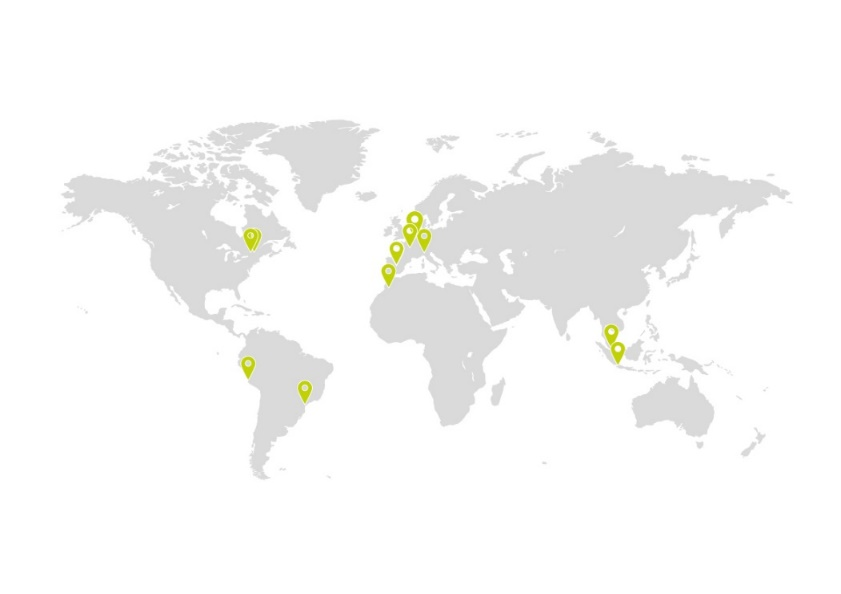
\includegraphics[width=0.4\textwidth]{altissia-presence-map.jpeg}
\end{wrapfigure}

\subsection{Panorema des offres et services}
\paragraph{}
Altissia s’est assigné comme mission, l’accès au plus grand nombre possible d’apprenants à l’apprentissage des langues et du langage sous une forme académique, structurante et ludique. Ses maîtres-mots sont la mobilité, l’immersion, la contextualisation, la personnalisation, l’Innovation, la Recherche et le Développement (IRD), la valorisation de la diversité et l’humanisme.

\paragraph{}
La porte d’entrée de tous les projets est une plateforme à la fois contextualisée et personnalisée en fonction de l’autorité contractante et de l’apprenant,
et globale puisque tous les projets englobent une grande variété de moyens,
tant présentiels que mobiles, pour permettre la réussite du projet.

\paragraph{}
Voici les principaux services qui composent les projets d’Altissia :
\begin{itemize}
    \item Une plateforme d’auto-formation, en ligne, dans 22 langues officielles de l’Union européenne
    \item Un outil adaptatif d’évaluation de niveau dans 24 langues
    \item Un service informel d’apprentissage des langues par l’actualité, renouvelé quotidiennement
    \item Le développement de contenus pédagogiques sur mesure
    \item Un réseau social d’échange linguistique
    \item Une solution de remédiation orthographique automatisée
    \item Des dispositifs multiples d’accompagnement de projet et des intervenants, combinant aussi bien les outils distanciels que présentiels.
\end{itemize}
\begin{figure}[ht]
    \centering
    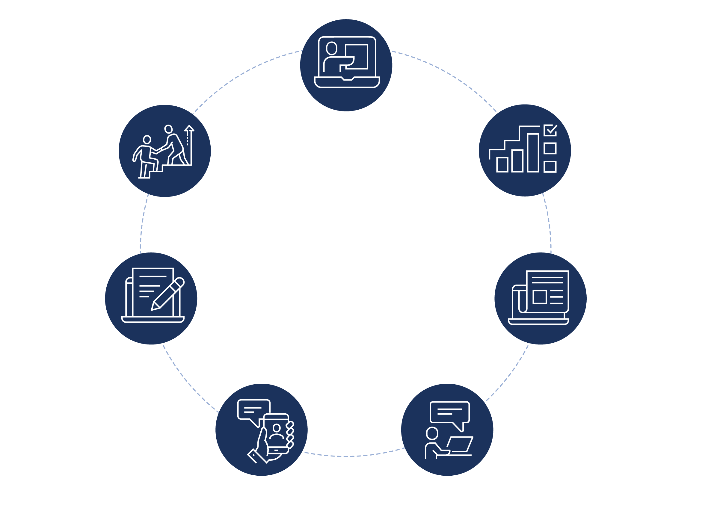
\includegraphics{altissia-services.png}
    \caption{Les multiples services proposés par Altissia}
    \label{fig:altissia-services}
\end{figure}

\subsection{Références}
\paragraph{}
Depuis quinze ans, Altissia œuvre à la mise en place, au déploiement et à la gestion de nombreux projets ambitieux d’évaluation et d’enseignement des langues à distance. Dans les lignes qui suivent, nous présentons quelques-unes des références majeures d’Altissia.

\subsubsection{Erasmus+ OLS}
\begin{wrapfigure}{R}{0.3\textwidth}
    \centering
    
\includegraphics[width=0.3\textwidth]{erasmusplus-logo.png}
\end{wrapfigure}
\paragraph{}
Le projet Erasmus+ OLS (\url{www.erasmusplusols.eu}) a été lancé par la Commission européenne en 2014 pour une période de sept ans. Ce projet consiste à créer, développer et promouvoir deux sous-projets, dans le cadre d’un consortium entre Altissia, le Centre de Langues (CLL\cite{cll_actualites_nodate}) et l’Université catholique de Louvain-la-Neuve (UCL).
 
\paragraph{}
Le premier sous-projet consiste à élaborer une plateforme de test de 24 langues pour tous les participants. Ce projet politique a pour mission de tester les participants au départ et au retour de leur séjour académique (de 1 à 12 mois) dans un établissement de l’un des pays de l’Union européenne.

\paragraph{}
Le second sous-projet consiste à élaborer, maintenir et promouvoir une plateforme d’apprentissage de 22 langues européennes. Cette plateforme doit permettre à l’apprenant d’améliorer toutes ses compétences linguistiques, par le biais de différentes activités, telles que des MOOC, des actualités internationales pédagogisées, des cours de groupe en visioconférence, etc.

\paragraph{}
Sur les sept années du projet, le nombre d’apprenants total est estimé à environ 4,5 millions.

\subsubsection{CNED}
\begin{wrapfigure}{R}{0.3\textwidth}
    \centering
    
\includegraphics[width=0.3\textwidth]{cned-logo.png}
\end{wrapfigure}
\paragraph{}
Le Centre national d’enseignement à distance, placé sous la tutelle du ministère de l’Éducation nationale fait confiance à Altissia depuis novembre 2014 pour la mise à disposition de contenus e-learning en anglais, espagnol, allemand, italien, néerlandais et français langue étrangère (FLE) pour les niveaux A1 à C1.

\paragraph{}
Les contenus proposés par Altissia sont intégrés au dispositif \#jeveuxparler, ainsi qu’aux parcours de plusieurs dizaines de filières BTS, conformes aux exigences des programmes officiels de ceux-ci. 

\subsubsection{Wallangues}
\begin{wrapfigure}{R}{0.3\textwidth}
    \centering
    
\includegraphics[width=0.3\textwidth]{images/wallangues-logo.jpeg}
\end{wrapfigure}
\paragraph{}
Wallangues (\url{www.wallangues.be}) a été lancé par la Région wallonne (Belgique) en 2011 pour une durée de quatre ans. Ce projet a pour but de donner un accès gratuit à tous les résidents wallons à l’apprentissage des trois langues nationales ainsi qu’à l’anglais. La mission de ce projet est d’améliorer la connaissance des langues pour renforcer la cohésion nationale, permettre un meilleur accès à l’emploi et à la mobilité et permettre une meilleure connaissance « de l’autre » et le respect de chacun.

\paragraph{}
Le public cible est d’environ 2,8 millions d’habitants. Ce projet a d’ailleurs été désigné par les citoyens comme la meilleure initiative du gouvernement wallon et, en 2015, le projet a été renouvelé pour cinq années supplémentaires, jusqu’en 2020. Une des particularités de ce projet est la collaboration et le partenariat inclusif entre le projet et les institutions publiques, telles que les ministères de l’Emploi et de la Formation continue et toutes les organisations semi-publiques en lien avec la jeunesse, l’emploi, les nouvelles technologies, l’alphabétisation et les ASBL (Associations sans but lucratif). L’ensemble des acteurs associés au projet partagent des missions qui ont un lien avec l’éducation, la formation, l’inclusion, l’intégration sociale, le sport et la culture.

\subsubsection{Mogilinguas - Mogi Das Cruzes -- Sao Paulo}
\begin{wrapfigure}{R}{0.3\textwidth}
    \centering
    
\includegraphics[width=0.3\textwidth]{mogi-linguas-logo.png}
\end{wrapfigure}
\paragraph{}
Mogilinguas (\url{www.mogilinguas.com.br}) est un projet qui a été lancé en 2017 par la préfecture de la ville de Mogi das Cruzes (Brésil) pour une durée de quatre ans. Ce projet a pour but de donner un accès gratuit à tous les résidents de la ville de Mogi das Cruzes à l’apprentissage de l’espagnol, de l’anglais et du français. 

\paragraph{}
Il s’agit d’un projet multifacette qui consiste à changer le paradigme de l’apprentissage au Brésil et à le mettre à disposition de tous les habitants. De multiples activités sont créées pour rendre le projet citoyen et pour que tous les habitants se l’approprient. Par exemple, une antenne Mogilinguas est installée dans la ville avec des points de rencontre itinérants. 

\paragraph{}
Le nombre de participants concernés est d’environ 420 000. 

\subsubsection{Des entreprises}
\begin{figure}[ht]
    \centering
    
\includegraphics[width=0.1\textwidth]{images/companies/ing-logo.jpeg}
    
\includegraphics[width=0.1\textwidth]{images/companies/swift-logo.jpeg}
    
\includegraphics[width=0.1\textwidth]{images/companies/total-logo.jpeg}
    
\includegraphics[width=0.1\textwidth]{images/companies/carrefour-logo.jpeg}
    
\includegraphics[width=0.1\textwidth]{images/companies/microsoft-logo.png}
    
\includegraphics[width=0.1\textwidth]{images/companies/belgacom-logo.jpeg}
    
\includegraphics[width=0.1\textwidth]{images/companies/ubisoft-logo.jpeg}
    
\includegraphics[width=0.1\textwidth]{images/companies/caterpillar-logo.jpeg}
    
\includegraphics[width=0.1\textwidth]{images/companies/solvay-logo.jpeg}
    
\includegraphics[width=0.1\textwidth]{images/companies/accenture-logo.jpeg}
    
\includegraphics[width=0.1\textwidth]{images/companies/dhl-logo.jpeg}
    
\includegraphics[width=0.1\textwidth]{images/companies/bpost-logo.jpeg}
    \caption{Quelques unes des entreprises qui ont choisi Altissia}
    \label{fig:companies-logo}
\end{figure}
Altissia compte parmi ses clients des entreprises de renoms telles que ING, Swift, Baxter, Total, Carrefour, Microsoft, Ubisoft, Proximus, Caterpillar, Solvay, Accenture, DHL, Bpost, etc.

\subsubsection{Éducation}
\begin{figure}[ht]
    \centering
    
\includegraphics[width=0.1\textwidth]{images/education/u-antwerpen-logo.jpeg}
    
\includegraphics[width=0.1\textwidth]{images/education/ucl-logo.jpeg}
    
\includegraphics[width=0.1\textwidth]{images/education/cll-logo.jpeg}
    
\includegraphics[width=0.1\textwidth]{images/education/u-st-louis-logo.jpeg}
    
\includegraphics[width=0.1\textwidth]{images/education/ichec-logo.png}
    
\includegraphics[width=0.1\textwidth]{images/education/ephec-logo.jpeg}
    
\includegraphics[width=0.1\textwidth]{images/education/uppna-logo.png}
    \caption{Quelques acteurs de l'éducation que Altissia aide dans leur mission}
    \label{fig:educations-logo}
\end{figure}
Altissia sert aussi des acteurs dans l'éducation tels que ICHEC, CLL, UCL, EPHEC, Upna, Universiteit Antwerpen, Université Saint-Louis, etc.

\subsection{Concurrents}
Altissia propose une offre complète et variée. Son offre se décline en plusieurs langues, est disponible sur plusieurs plateformes, prends diverses formes et occupe toutes les facettes du marchés (B2B, B2I, B2E et B2C).
De ce fait, de nombreux concurrents existent mais sur des segments restreints de l'espace qu'occupe Altissia.

Ses concurrents les plus directs sont Rosetta Stone, 7 Speaking, GOFluent, Speexx et Télélangue.

\subsection{Service cible de l'application}
\label{ssec:target-service}
\paragraph{}
L'application sera utilisée par le service linguistique et informatique qui sont conjointement responsables du contenu de cours
et du développement des plate-formes de cours.
Ces deux services comptabilisent une quarantaine de personnes et comporte des profils de linguistes, développeurs informatiques,
concepteurs d'interfaces utilisateur, administrateurs systèmes, chefs de projets et analystes fonctionnels.

\paragraph{}
Le personnel IT s'occupera de configurer l'outil tandis que les utilisateurs principaux seront les chefs de projets ainsi que les linguistes.


\section{La demande initiale}
\label{sec:initial-request}

    \paragraph{}
Des tâches sont actuellement effectuées par une bibliothèque de scripts \href{https://ant.apache.org/}{Apache Ant}\footnote{Apache Ant est un outil permettant de construire une application Java à partir de son code source. Une alternative plus connue est \href{https://maven.apache.org/}{Apache Maven}.}.
Certaines sont effectuées avec des scripts codés en \href{https://www.python.org/}{Python}\footnote{Langage de programmation très populaire pour créer des scripts.}.
Enfin d'autres sont réalisées avec le socle d'application\footnote{Socle d'application ou \textit{Framework} en anglais; ensemble cohérent de composants logiciels permettant de construire les fondations d'un logiciel\cite{wikipedia_framework_2019}.} Spring\footnote{Spring est un socle d'application Java.} Batch\footnote{Spring Batch est un composant du \textit{Framework} Spring permettant un traitement par lots de grande quantité de données.}.

\paragraph{}
Malheureusement, seuls des développeurs sont capables d'utiliser ces outils.
En effet, ils ne disposent pas d'interface graphique ou de connexion avec des programmes classiques\footnote{Il est existe une connexion entre certains modules Apache Ant et Excel mais c'est loin d'être ergonomique et est finalement peu utilisé.}.
De plus, rien ne centralise ces applications, ce qui ne facilite pas non plus la vie des programmeurs.
Ces programmes ont été écris au moment où ils étaient nécessaire sans trop de pensées vers l'architecture globale du système applicatif futur.
Ce qui rends ces applications assez chers à maintenir et peu plaisantes à faire évoluer.

\paragraph{}
Le but principal du nouveau logiciel est de centraliser tous ces processus, fournir un cadre les rendant plus facile à développer et à faire évoluer et permettant leur utilisation au travers d'une interface graphique par un acteur métier.


\section{Les produits existants}
\label{sec:existing-products}

    \section{Les produits existants}
\label{sec:existing-products}

\paragraph{}
Le coeur du projet consiste à implémenter les règles logiques qui régissent le contenu de cours et de tests d'Altissia.
Il n'existe donc aucun produit existant qui fasse cela.

\paragraph{}
Toutefois, il est possible de choisir de s'appuyer sur certains produits existants pour une partie des fonctionnalités.
Il y a notamment une partie de l'application qui doit gérer l'exécution des différentes tâches, reporter leur statut, tenir un historique, etc.
Ces responsabilités tombent sous le coup d'un planificateur de tâches.
% Est-ce que je peux uniquement utiliser le front de Rundeck ou dois-je créer un front intermédiaire qui appelle l'API de rundeck ?

\paragraph{}
Des exemples connus sont: Ansible, Rundeck, Salt, Chef et Fabric.
Il se trouve que Altissia utilise justement Rundeck pour automatiser ses déploiements\fnmark.
Il n'y a donc pas lieu d'acheter des licences pour une alternative ou de s'y former.

\fntext{Dans le contexte du développement informatique, le déploiement est l'acte de rendre une application disponible aux utilisateurs.}

\paragraph{}
Rundeck se présente sur sa page d'accueil\cite{rundeck_rundeck_nodate}, traduit de l'anglais:
\begin{displayquote}
Transformez vos procédure opérationnelles en tâches disponibles en libre service. Donnez le contrôle et la transparence aux autres en toute sécurité.
\end{displayquote}
Ce qui est bien le but recherché.
Rendre disponible des processus existants et donner le contrôle aux acteurs métiers. 



	\chapter{Cahier des charges}
	\label{ch:specifications}

		\paragraph{}
Le besoin est né du constat de la lourdeur de processus existants.
Une solution existe mais ne satisfait pas.

D'une part, les personnes à la base des besoins métiers souffrent de résultats mitigés et longs à attendre.
D'autre part, les développeurs doivent exécuter des demandes dont les exécutions sont manuelles et répétitives.

\paragraph{}
La ligne directrice sera donc d'automatiser de manière complète des processus existants et de faire en sorte qu'ils
puissent être menés à bien par la seule personne ayant besoin du résultat de ces processus.

\section{Élaboration}
\label{sec:elaboration}

    \section{Élaboration}
\label{sec:elaboration}

L'élaboration de ce cahier des charges s'est faite en deux phases. 
Dans un premier temps, j'ai participé à des réunions avec Grégory, Renaud et Sophie afin de démarrer le projet. 
Et dans un second temps, nous avons ajouté et adapté des fonctionnalités au fur et à mesure que le projet a avancé.

\paragraph{}
Altissia travaille selon les principes agiles\fnmark et plus précisément la méthodologie SCRUM\fnmark.
Ces principes sont nés d'un constat sur les projets informatiques, pour la majorité échoue\cite{standish_standish_nodate} et la plupart du temps c'est parce que les besoins sont mal définis ou parce que la communication entre les parties prenantes est mauvaise (voir figure \ref{fig:why-projects-fails}).

\begin{figure}[ht]
    \centering
    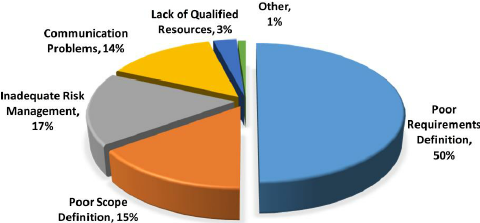
\includegraphics[scale=.8]{images/why-projects-fail.png}
    \caption{Role of Requirements in Software Project Failures. Source: ESI International Survey of 2000 Business Professionals, 2005.}
    \label{fig:why-projects-fails}
\end{figure}

\fntext{Dans le contexte du développement logiciel, l'agilité définit un cadre de travail\cite{noauthor_methode_2018}.
Un point central est le développement par itération dont chacune produit un résultat critiquable par le client.
Ceci a pour but de limiter les efforts potentiellement perdus si le résultat ne correspond pas aux attentes.}
\fntext{Une méthode Agile spécifique qui a la particularité d'organiser le travail sous forme d'échéances à court termes et répétées que l'on appelle les sprints\cite{noauthor_guide_2013}.}

\paragraph{}
Pour répondre à ces enjeux, le service informatique d'Altissia a adopté la méthode SCRUM.
Cela consiste à travailler de manière itérative, de produire des résultats intermédiaires utilisables fréquents, d'impliquer les différents acteurs, d'obtenir leurs commentaires et d'adapter la direction du projet selon ceux-ci.

\paragraph{}
C'est donc pour cela que le cahier des charges n'est pas complet et définitif au début du projet mais qu'il s'étoffe au fur et à mesure.

\subsection{Les interviews}
\label{subsec:interviews}

    En un premier temps, j'ai eu une interview avec Grégory pour définir le besoin général et le contexte qui l'entoure. 
    
    Ensuite, j'ai eu une réunion avec Renaud et Sophie.
    A deux, ils ont défini précisément la problématique des outils existants.
    Renaud connaît très bien l'outil que l'on veut remplacer, Altissia launcher, il m'a expliqué les difficultés rencontrées pendant son développement et comment il a terminé dans son état actuel.
    
    % Elaborer sur les manquements d'Altissia launcher ? On en parle un peu dans l'intro donc pas sur que ça soit nécessaire.
    Sophie a établi quelles sont les manquements du logiciel actuel qu'il faudrait palier et quelles nouvelles fonctionnalités elle voudrait ajouter.

    \paragraph{}
    Une interview avec le directeur technique m'a permis d'établir comment la nouvelle application intéragira avec les applications existantes.

    L'application sera hébergée sur le réseau de travail de l'entreprise.
    Elle doit supporter certaines fonctionalités mais pas l'authentification utilisée par nos microservices en tant que telle.
    Afin de donner accès aux ressources protégées, Altissia créera une version personnalisée\footnotemark de l'application.
    \footnotetext{La personnalisation signifie la reprise du code source afin d'y ajouter les fonctionalités désirées.}

    Ainsi, l'application sera constitué de quatres sortes de composants:
    \begin{itemize}
        \item Une application web cliente Angular qui lui permet d'intéragir avec les utilisateurs.
        \item Une application web server qui permet de communiquer avec les ressources réseaux.
        Celle-ci sera personnalisée afin d'implémenter l'authentification d'Altissia.
        \item Une librairie d'automatisation qui gère l'exécution des tâches et leur journalisation.
        \item Des multiples modules qui chacun permettent de définir une ou plusieurs tâches.
    \end{itemize}

    \paragraph{}
    Renaud, un développeur backend expérimenté, m'a expliqué le défi que sera la libraire d'automatisation de tâches.
    Il faut supporter la définition d'une tâche, l'asynchronicité de son exécution, la possibilité d'exécutions répétées,
    l'utilisation de ressources partagées et la réutilisabilité des tâches.

    Je dois lui proposer une architecture qui permet de relever tous ces défis.

    \paragraph{}
    Sophie, une cheffe de projet qui s'occupe notamment de la publication du contenu des cours et tests de niveaux,
    a défini quel serait le périmètre de l'application.
    Le but est de ne pas implémenter des fonctionalités qui font déjà l'objet de développements prévus ou en cours.

    La fonctionalité qui obtient la priorité pour le moment est la validation du contenu des fichiers Excel des questions du test de niveau.
    Celle-ci est fort demandée et sa complexité est moyenne.
    Elle permettrait de se faire une idée plus précise de ce que l'application pourrait apporter.

    \paragraph{}
    Le directeur technique et moi-même sommes mis d'accord pour une réunion bi-hebdomadaire.
    Je dois organisé une nouvelle réunion avec Renaud pour lui présenter mon plan d'architecture.
    Je verra Sophie dans un moi ou deux pour passer en revue le premier délivrable et discuter des prochains délivrables.

\subsection{Les demandes clients}
\label{subsec:customer-requests}

    La première fonctionalité sera la validation des fichiers Excel des questions de test de niveaux.
    Cette validation comprends les points suivants:
    \begin{enumerate}
        \item La correspondance à une expression régulière.
        \item L'unicité des valeurs au sein d'une colonne.
        \item La cohérence entre deux colonnes (Si la colonne type a la valeur audio, alors la colonne son doit avoir une valeur).
        \item La présence d'une colonne.
        \item L'absence d'impact de colonnes superflues.
        \item L'appartenance à un ensemble de comparaison.
    \end{enumerate}

\subsection{Les propositions au client}
\label{subsec:proposals-to-customer}

    J'ai proposé de n'implémenter que la présence d'une colonne pour la première itération.
    C'est évidemment trop peu pour réaliser un scénario complet mais l'objectif est la mise en place des différents composants logiciels.
    Ainsi, une fois cette première itération accomplie, on pourra juger de la pertinence de la solution choisie.


\section{Lots d'informations identifiés}
\label{sec:identified-information-packages}

    TODO

\section{Les acteurs de l'environnement d'exploitation de l'application}
\label{sec:application-operation-actors}

    TODO

\section{Définition de la première version de l'application}
\label{sec:first-version-definition}

    TODO

\section{Perspectives d'évolution pour une version ultérieure}
\label{sec:future-release-outlook}

    TODO


	\chapter{Analyse}
	\label{ch:analysis}

		TODO

	\chapter{Réalisation}
	\label{ch:implementation}

		TODO

	\chapter{Évolutions immédiates pressenties}
	\label{ch:next-steps}

		TODO

	\chapter{Évaluation du travail}
	\label{ch:auto-critic}

		TODO

	\chapter{Conclusion}
	\label{ch:conclusion}

		TODO
		
	\begin{appendix}
\chapter{Documentation d'un processus d'Altissia launcher}
\label{ch:altissia-launcher-doc}

\paragraph{}
Par soucis de confidentialité, je n'ai finalement pas pu joindre cet extrait de code.

\paragraph{}
Son but était de monter que c'était un processus complexe à suivre et non intuitif.
\chapter{Extrait d'un Excel des questions de test de niveaux}
\label{ch:leveltest-sample}

\paragraph{}
Les questions de tests de niveaux sont des objets complexes que l'on modélise avec plus d'une quarantaine de champs.
J'ai copié un extrait simplifié ci-dessous.

La longueur d'un seul enregistrement était trop long pour tenir sur une feuille, je le présente ici sous forme vertical en rappellant l'entête pour chaque enregistrement.
Dans un soucis de clarté et de lisibilité j'ai activé le retour à la ligne automatique et j'ai remplacé les traits de soulignement avec des espaces pour permettre le retour à la ligne.

\begin{table}[ht]
\begin{tabular}{p{5cm}|p{8cm}}
 & Question 1 \\ \hline
UUID & 2014020611193800100 \\
UUID multipleChoice & 2014020611203209500 \\
MultipleChoice & 1 \\
Open & 0 \\
studyLg & EN \\
locale & EN GB \\
level EU & A2 \\
test name & GRAMMAR \\
online & 1.0 \\
topic tags & (C1 -\textgreater{}) Legal matters \\
grammar tags 1 &  \\
grammar tags 2 &  \\
functions tags &  \\
status & 5-validated \\
type & multiple choice 4 options \\
name & EN 92 \\
instruction multipleChoice four options & Choose the right answer. \\
instruction key & la choose instruction \\
question & - Where are the keys {[}GAP{]} I left on the desk? \\
GAP 1 correct 1 & which \\
GAP 1 incorrect 1 & who \\
GAP 1 incorrect 2 & whom \\
GAP 1 incorrect 3 & those \\
UUID sound & NA \\
sound base reference & NA \\
status sound & NA
\end{tabular}
\end{table}

\begin{table}[ht]
\begin{tabular}{p{5cm}|p{8cm}}
 & Question 2 \\ \hline
UUID & 2014020611232012500 \\
UUID multipleChoice & 2015080312593955700 \\
MultipleChoice & 1 \\
Open & 0 \\
studyLg & EN \\
locale & EN GB \\
level EU & A1 \\
test name & GRAMMAR \\
online & 1.0 \\
topic tags & (A1-\textgreater{}) work and jobs \\
grammar tags 1 & gerund forms \\
grammar tags 2 & passive voice \\
functions tags &  \\
status & 5-validated \\
type & multiple choice 4 options \\
name & EN 94 \\
instruction multiple Choice four options & Choose the right answer. \\
instruction key & la choose instruction \\
question & - I'm going to swim in the sea; do you want to come?- I would love to, but it's impossible for me because I {[}GAP{]} swim! \\
GAP 1 correct 1 & can't \\
GAP 1 incorrect 1 & haven't \\
GAP 1 incorrect 2 & must \\
GAP 1 incorrect 3 & needn't \\
UUID sound & NA \\
sound base reference & NA \\
status sound & NA
\end{tabular}%
\end{table}

\chapter{Extrait du code d'Altissia launcher}
\label{ch:altissia-launcher-code}

\paragraph{}
Par soucis de confidentialité, je n'ai finalement pas pu joindre cet extrait de code.

\paragraph{}
Il avait pour but d'illustrer la complexité de la tâche qu'il fallait relevé.
Ce code était complexe et a été remplacé par un code élégant.

\chapter{La classe \textit{Language.java}}
\label{ch:language-java}

\paragraph{}
Cette classe est une reproduction simplifiée d'une classe utilisée par les services d'Altissia pour manipuler la notion de langue.
L'intérêt est de constater que ce n'est pas une simple liste de langues mais qu'elle définit une nomenclature stricte et classe ses sujets selon les critères d'utilisation.
Toutes langues listée ici est une langue d'interface et certaines sont des langues d'étude.

\paragraph{}
Cela se comprends car il est beaucoup plus difficile de créer le contenu d'apprentissage que traduire les textes des interfaces.
De plus, afficher du contenu de cours dans une langue nécessite d'avoir fait le travail requis pour afficher cette langue.
Il ne reste donc en comparaison aucun effort à faire pour transformer une langue d'étude en une langue d'interface.
Et cet effort est systématiquement fait.

\lstinputlisting[language=java]{pages/appendix/Language.java}
\end{appendix}

	\printbibliography

	\clearpage
\newpage
\pagenumbering{gobble}
\null
\clearpage
 % last page must be empty
\end{document}
